\documentclass[
paper=a4,                       % paper size
fontsize=11pt,                  % font size
headinclude=false,              % header does not belong to the text
footinclude=false,              % footer does not belong to the text
pagesize,                       % set the pagesize in a DVI document
]{scrartcl}

% Copyright (C) 2010,2011,2012 The ESPResSo project
% Copyright (C) 2002,2003,2004,2005,2006,2007,2008,2009,2010
%  Max-Planck-Institute for Polymer Research, Theory Group
%  
% This file is part of ESPResSo.
%   
% ESPResSo is free software: you can redistribute it and/or modify it
% under the terms of the GNU General Public License as published by the
% Free Software Foundation, either version 3 of the License, or (at your
% option) any later version.
%  
% ESPResSo is distributed in the hope that it will be useful, but
% WITHOUT ANY WARRANTY; without even the implied warranty of
% MERCHANTABILITY or FITNESS FOR A PARTICULAR PURPOSE.  See the GNU
% General Public License for more details.
%  
% You should have received a copy of the GNU General Public License
% along with this program.  If not, see <http://www.gnu.org/licenses/>.
%
\usepackage[draft]{varioref}    % defines \vref
\usepackage{hyperref}           % automatically creates links when
                                % using pdflatex, defines \url
\usepackage{ifpdf}              % defines \ifpdf
\usepackage{graphicx}           % handles graphics
\usepackage{color}              % use colors

\usepackage{amsmath}

\usepackage{verbatim}           % required for \verbatim and \endverbatim
\usepackage{fancyvrb}
\usepackage{calc}               % compute length
\usepackage{ifthen}             % provide ifthen
\usepackage{xspace}
\usepackage{units}
\usepackage[numbers]{natbib}

% For building the distribution docs, disable todo boxes.
%\usepackage[disable]{todonotes}
\usepackage{todonotes}

\newcommand{\es}{\mbox{\textsf{ESPResSo}}\xspace}
\newcommand{\ie}{\textit{i.e.}\xspace}
\newcommand{\eg}{\textit{e.g.}\xspace}
\newcommand{\etal}{\textit{et al.}\xspace}

\newcommand{\codebox}[1]%
{\texttt{#1}}

\DefineVerbatimEnvironment{code}{Verbatim}%
{commandchars=\\\{\}}
\makeatletter
\newenvironment{tclcode}
{%
  \addtolength{\linewidth}{-2em}% set the line length
  \@minipagetrue%%%DPC%%%
  \@tempswatrue%%%DPC%%%
  \hsize=\linewidth%
  \setbox0=\vbox\bgroup\verbatim
}{\endverbatim
  \unskip\setbox0=\lastbox%%%DPC%%%
  \egroup
  \par%
  \noindent\hspace{1em}%
  \codebox{\box0}%
  \par\noindent%
}
\makeatother

% \newcommand{\todo}[1]{
%   \marginpar{%
%     \setlength{\fboxrule}{1pt}
%     \fcolorbox{red}{yellow}{%
%       \parbox{\marginparwidth-2\fboxrule-2\fboxsep}{%
%         \bf\raggedright\scriptsize #1%
%       }%
%     }%
%   }%
% }

\makeatletter
\renewcommand{\minisec}[1]{\@afterindentfalse \vskip 1.5ex
  {\parindent \z@
    \raggedsection\normalfont\sffamily\itshape\nobreak#1\par\nobreak}%
  \@afterheading}
\makeatother

\newcommand{\esptitlehead}{
  \titlehead{
    \begin{center}
      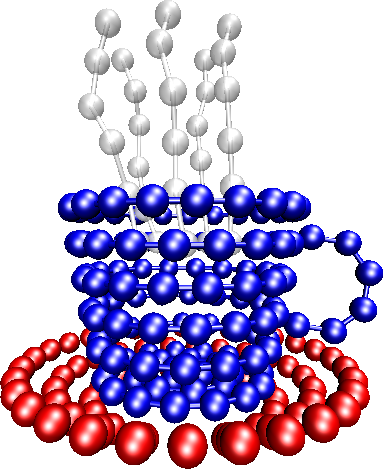
\includegraphics[width=5cm]{logo/transparentbg}
    \end{center}
  }
}


%% Grafikpakete
\usepackage{graphicx}%


\usepackage{verbatim}

% How to diplay ESPResSo commands in flowing text. Larger code segments
% should be put inside boxes.
% \newcommand{\EScmd}[1]{\texttt{\textbf{#1}}}

\usepackage{listings}

\definecolor{codebg}{rgb}{0.95,0.95,0.95}
\definecolor{codeframe}{gray}{0.5}
\definecolor{codeshadow}{gray}{0.7}
\definecolor{codenumber}{rgb}{0.58,0,0.82}
\definecolor{pblau}{rgb}{0.09375,0.19921875,0.4296875}

\usepackage{listings}
\lstset{
  basicstyle=\ttfamily,
  keywordstyle=\bfseries\ttfamily\color[rgb]{0.65,0.16,0.18},
  identifierstyle=\ttfamily\color{pblau},
  commentstyle=\color[rgb]{0.133,0.545,0.133},
  stringstyle=\ttfamily\color[rgb]{0.627,0.126,0.941},
  showstringspaces=false,
  tabsize=2,
  breaklines=true,
  prebreak = \raisebox{0ex}[0ex][0ex]{\ensuremath{\hookleftarrow}},
  breakatwhitespace=false,
  numberstyle=\footnotesize \sf,
  numbers=none,
  stepnumber=1,
  numbersep=1.5em,
  xleftmargin=2.7em,
  framexleftmargin=2.7em,
  aboveskip={1\baselineskip},
  belowskip={1\baselineskip},
  columns=fixed,
  upquote=true,
  extendedchars=true,
  frame=shadowbox,
  rulesepcolor=\color{codeshadow},
  rulecolor=\color{codeframe},
  backgroundcolor=\color{codebg},
  mathescape=true
}


\begin{document}

\esptitlehead

\title{Setting up \es{}
\ifdefined\esversion%
\thanks{For \es \esversion}%
\fi%
}
\author{}

\maketitle

\section{Introduction}
\es{} is distributed as source code because this allows the user to disable features that are mutually exclusive or would otherwise decrease the performance unnecessarily. Users typically  build a custom \es{} binary for a specific simulation, containing only the minimal set of features required for this application. This tutorial will guide you through this whole process  from obtaining the source code of the development version, to configuring and building binaries, to compiling the documentation.

\section{Getting the Source Code}
\subsection{Download the Source Code for the Development Version}
%
For the development version, first clone the \es{} reposity from github by running
\begin{lstlisting}[language=bash]
git clone https://github.com/espressomd/espresso.git
\end{lstlisting}
%
in a terminal. This creates a local copy of the current \es{} repository in the folder \verb!espresso!.
Enter the newly create directory using
\begin{lstlisting}[language=bash]
cd espresso
\end{lstlisting}
It is recommended to create a \verb!build! directory with
\begin{lstlisting}[language=bash]
mkdir build && cd build
\end{lstlisting}
that will contain all the data that is generated in the following. Next, run
\begin{lstlisting}[language=bash]
cmake ..
\end{lstlisting}
to configure the build system.

%           %%% NOT AVAILABLE FOR PYTHON YET %%%
% \subsection{Release Version}
% The \es{} releases can be downloaded from the \es{} website at\\
% \verb!http://espressomd.org/wordpress/download/!.
% After downloading the latest version unpack it by running
% \begin{lstlisting}[language=bash]
%   tar xfv espresso-X.Y.Z.tar.gz
% \end{lstlisting}
% where X Y an Z have to be replaced with the actual version numbers.

\subsection{Compiling \es{}}
%From here on the procedure is the same for both versions.
Now compile \es from within the build subfolder with the command
%
\begin{lstlisting}[language=bash]
make -j 8
\end{lstlisting}
With the option \verb!-j! you can specify how many threads are used for the make process which will speed up the compilation.
%
It is good to know that you can maintain several build folders with different feature sets using the same \es{} source folder. They don't have to reside within the source directory.
%
If you have installed the curses frontend to \verb!cmake! you can see and modify the build options graphically by running
\begin{lstlisting}[language=bash]
ccmake ..
\end{lstlisting}
before the \verb!make! command. \es{} requires a number of external libraries depending on the feature set you plan to use. Most, if not all of these libraries will be available through your Linux distribution's repositories. If you manually install dependencies in a non-standard location, you have to specify this location with the \texttt{ccmake} command. If, for example, you plan to use GPU features and your cuda toolkit is not located under \texttt{/usr/local/cuda}, you will have to specify its location explicitly. Remember, after you changed configurations with \verb!ccmake!, the new configuration set have to be built by using the \verb!make -j 8! command again.
%
This produces an executable named \verb!pypresso! in the build directory which can be run by
\begin{lstlisting}[language=bash]
./pypresso
\end{lstlisting}

\subsection{Documentation}

For the development code and upcoming releases see the Online Documentation for
ESPResSo with python at \url{http://espressomd.org/html/doc/index.html}.

As an expert option, you can locally create this html documentation by running
\begin{lstlisting}[language=bash]
make sphinx
\end{lstlisting}
in your build directory. The resulting web pages can then be browsed by opening \texttt{build/doc/spinx/html/index.html}.

\subsection{Configuring features}
%
After successfully running the \verb!cmake! script, your build folder will contain a file \\ \texttt{myconfig-sample.hpp}. Create a copy of this file called \texttt{myconfig.hpp} by executing
%cd ..
\begin{lstlisting}[language=bash]
cp myconfig-sample.hpp myconfig.hpp
\end{lstlisting}
%
Then uncomment the respective lines in \texttt{myconfig.hpp} (by removing the leading slashes) to enable features your simulation requires. The User's Guide contains information about required features for every \es{} command.
When you activate or deactivate features, you have to \verb!rebuild! the binaries by running
%
\begin{lstlisting}[language=bash]
make -j 8
\end{lstlisting}
%
in the build directory.

\end{document}
